\documentclass[tikz,border=5pt]{standalone}
\usepackage{tikz}

\begin{document}
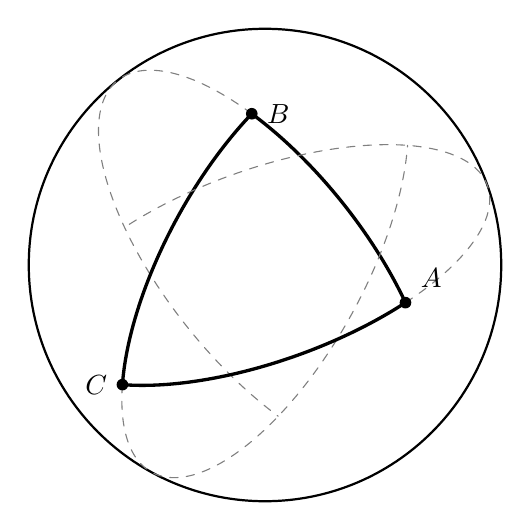
\begin{tikzpicture}[scale=3, line cap=round, line join=round]

  % Unit sphere outline (orthographic projection from above)
  \draw[thick] (0,0) circle (1);

  % Choose three vertices on the front hemisphere by latitude/longitude (degrees)
  \pgfmathsetmacro{\latA}{52}
  \pgfmathsetmacro{\lonA}{-15}
  \pgfmathsetmacro{\latB}{50}
  \pgfmathsetmacro{\lonB}{95}
  \pgfmathsetmacro{\latC}{38}
  \pgfmathsetmacro{\lonC}{220}

  % Convert to 3D unit vectors (x=cosf cos?, y=cosf sin?, z=sinf)
  \pgfmathsetmacro{\Ax}{cos(\latA)*cos(\lonA)}
  \pgfmathsetmacro{\Ay}{cos(\latA)*sin(\lonA)}
  \pgfmathsetmacro{\Az}{sin(\latA)}

  \pgfmathsetmacro{\Bx}{cos(\latB)*cos(\lonB)}
  \pgfmathsetmacro{\By}{cos(\latB)*sin(\lonB)}
  \pgfmathsetmacro{\Bz}{sin(\latB)}

  \pgfmathsetmacro{\Cx}{cos(\latC)*cos(\lonC)}
  \pgfmathsetmacro{\Cy}{cos(\latC)*sin(\lonC)}
  \pgfmathsetmacro{\Cz}{sin(\latC)}

  % Helper: draw the great-circle arc between P and Q (shorter arc solid, opposite half dashed)
  \newcommand{\DrawGCArc}[9]{%
    % Inputs: nx ny nz, Px Py Pz, Qx Qy Qz (n is plane normal)
    \pgfmathsetmacro{\nx}{#1}\pgfmathsetmacro{\ny}{#2}\pgfmathsetmacro{\nz}{#3}
    \pgfmathsetmacro{\px}{#4}\pgfmathsetmacro{\py}{#5}\pgfmathsetmacro{\pz}{#6}
    \pgfmathsetmacro{\qx}{#7}\pgfmathsetmacro{\qy}{#8}\pgfmathsetmacro{\qz}{#9}
    \pgfmathsetmacro{\plen}{sqrt(\nx*\nx + \ny*\ny)} % |projection of n onto xy|
    % Orthonormal basis (u,v) for the great-circle plane
    \pgfmathsetmacro{\ux}{-\ny/\plen}
    \pgfmathsetmacro{\uy}{ \nx/\plen}
    \pgfmathsetmacro{\uz}{ 0}
    \pgfmathsetmacro{\vx}{-\nz*\nx/\plen}
    \pgfmathsetmacro{\vy}{-\nz*\ny/\plen}
    \pgfmathsetmacro{\vz}{ \plen}
    % Endpoint parameters on the circle r(t) = u cos t + v sin t
    \pgfmathsetmacro{\cuP}{\px*\ux + \py*\uy + \pz*\uz}
    \pgfmathsetmacro{\cvP}{\px*\vx + \py*\vy + \pz*\vz}
    \pgfmathsetmacro{\tP}{atan2(\cvP,\cuP)}
    \pgfmathsetmacro{\cuQ}{\qx*\ux + \qy*\uy + \qz*\uz}
    \pgfmathsetmacro{\cvQ}{\qx*\vx + \qy*\vy + \qz*\vz}
    \pgfmathsetmacro{\tQ}{atan2(\cvQ,\cuQ)}
    % Shorter difference in [-180,180]
    \pgfmathsetmacro{\dAng}{mod(\tQ-\tP+540,360)-180}
    % Draw short (front) arc and opposite (back) half
    \draw[very thick]
      plot[domain=\tP:\tP+\dAng, samples=140, variable=\t]
        ({\ux*cos(\t)+\vx*sin(\t)}, {\uy*cos(\t)+\vy*sin(\t)});
    \draw[gray, dashed]
      plot[domain=\tP+\dAng:\tP+\dAng+180, samples=140, variable=\t]
        ({\ux*cos(\t)+\vx*sin(\t)}, {\uy*cos(\t)+\vy*sin(\t)});
  }

  % Great-circle normals for edges are n = P x Q (unitized)
  % AB
  \pgfmathsetmacro{\nABx}{\Ay*\Bz - \Az*\By}
  \pgfmathsetmacro{\nABy}{\Az*\Bx - \Ax*\Bz}
  \pgfmathsetmacro{\nABz}{\Ax*\By - \Ay*\Bx}
  \pgfmathsetmacro{\nABn}{sqrt(\nABx*\nABx + \nABy*\nABy + \nABz*\nABz)}
  \pgfmathsetmacro{\nABx}{\nABx/\nABn}
  \pgfmathsetmacro{\nABy}{\nABy/\nABn}
  \pgfmathsetmacro{\nABz}{\nABz/\nABn}
  % BC
  \pgfmathsetmacro{\nBCx}{\By*\Cz - \Bz*\Cy}
  \pgfmathsetmacro{\nBCy}{\Bz*\Cx - \Bx*\Cz}
  \pgfmathsetmacro{\nBCz}{\Bx*\Cy - \By*\Cx}
  \pgfmathsetmacro{\nBCn}{sqrt(\nBCx*\nBCx + \nBCy*\nBCy + \nBCz*\nBCz)}
  \pgfmathsetmacro{\nBCx}{\nBCx/\nBCn}
  \pgfmathsetmacro{\nBCy}{\nBCy/\nBCn}
  \pgfmathsetmacro{\nBCz}{\nBCz/\nBCn}
  % CA
  \pgfmathsetmacro{\nCAx}{\Cy*\Az - \Cz*\Ay}
  \pgfmathsetmacro{\nCAy}{\Cz*\Ax - \Cx*\Az}
  \pgfmathsetmacro{\nCAz}{\Cx*\Ay - \Cy*\Ax}
  \pgfmathsetmacro{\nCAn}{sqrt(\nCAx*\nCAx + \nCAy*\nCAy + \nCAz*\nCAz)}
  \pgfmathsetmacro{\nCAx}{\nCAx/\nCAn}
  \pgfmathsetmacro{\nCAy}{\nCAy/\nCAn}
  \pgfmathsetmacro{\nCAz}{\nCAz/\nCAn}

  % Draw the three geodesic edges (great-circle short arcs)
  \DrawGCArc{\nABx}{\nABy}{\nABz}{\Ax}{\Ay}{\Az}{\Bx}{\By}{\Bz}
  \DrawGCArc{\nBCx}{\nBCy}{\nBCz}{\Bx}{\By}{\Bz}{\Cx}{\Cy}{\Cz}
  \DrawGCArc{\nCAx}{\nCAy}{\nCAz}{\Cx}{\Cy}{\Cz}{\Ax}{\Ay}{\Az}

  % Vertex markers and labels (projected positions)
  \fill (\Ax,\Ay) circle (0.7pt) node[above right=2pt] {$A$};
  \fill (\Bx,\By) circle (0.7pt) node[right=2pt]       {$B$};
  \fill (\Cx,\Cy) circle (0.7pt) node[left=2pt]        {$C$};

\end{tikzpicture}
\end{document}
